% ============================================================
% 7. Design
% ============================================================
\chapter{Design}\label{ch:design}

\section{BCE Architecture (VOPC)}

CiboAmico follows the \textbf{Boundary--Control--Entity} pattern. The VOPC
(view of participating classes) respects the following rules:
\begin{itemize}
    \item each use case owns exactly \textbf{one application controller};
    \item boundaries exchange data with controllers \textbf{exclusively via
    beans (DTO)}: no entity reaches the view;
    \item controllers are \textbf{stateless}: the current user is passed as a
    parameter by the view, which resolves it from the session singleton
    (SessionManager);
    \item business logic resides in the entities.
\end{itemize}

The final model is summarised in Table~\ref{tab:vopc}. The boundary
column reports the real JavaFX view classes; the bean column lists the DTOs
interposed between boundary and control (bean-only rule); the adapters are
the technical boundaries that mediate the interaction with the external
systems. The Payment Service is declared as an external actor of UC-04 for
completeness but is simulated in code (out of the evaluation scope, see
Implementation Remarks in Chapter~\ref{ch:intro}); the email notification
(UC-04/UC-06) is mediated by the \texttt{JakartaMailAdapter}.

\begin{table}[H]
\centering
\caption{BCE classes (1 controller per use case).}
\label{tab:vopc}
\begin{tabular}{@{}lllll@{}}
\toprule
\textbf{UC} & \textbf{Boundary} & \textbf{Bean} & \textbf{Control} & \textbf{Main Entities} \\
\midrule
UC-01 & InventarioView & ProdottoBean & GestisciInventarioController & ProdottoInventario \\
UC-02 & RicetteView & RicettaBean & TrovaRicetteController & Ricetta, ProdottoInventario \\
UC-03 & ListaSpesaView & RicettaBean & GestisciListaSpesaController & Ricetta, Ingrediente \\
UC-04 & MarketplaceView & OrdineBean & OrdinaProdottoController & Ordine, Prodotto \\
UC-05 & CatalogoVenditoreView & ProdottoBean & GestisciCatalogoVenditoreController & Prodotto, RuoloVenditore \\
UC-06 & OrdiniRicevutiView & OrdineBean & GestisciOrdiniRicevutiController & Ordine \\
UC-07 & RicetteNutrizionistaView & RicettaBean & GestisciRicetteNutrizionistaController & Ricetta, RuoloNutrizionista \\
UC-08 & AdminView & RicettaBean, UtenteBean & ApprovazioneController & RuoloVenditore, Ricetta \\
UC-11 & LoginView & AutenticazioneBean & AutenticazioneController & Utente \\
\bottomrule
\end{tabular}
\end{table}

\section{Design-Level Class Diagram}

The design-level class diagram refines the VOPC with the real Java classes,
their attributes with effective types, method signatures and the persistence
interfaces. For readability it shows the core of UC-04 and the key
architectural patterns; the remaining controllers follow the same shape.

\begin{figure}[H]
\centering
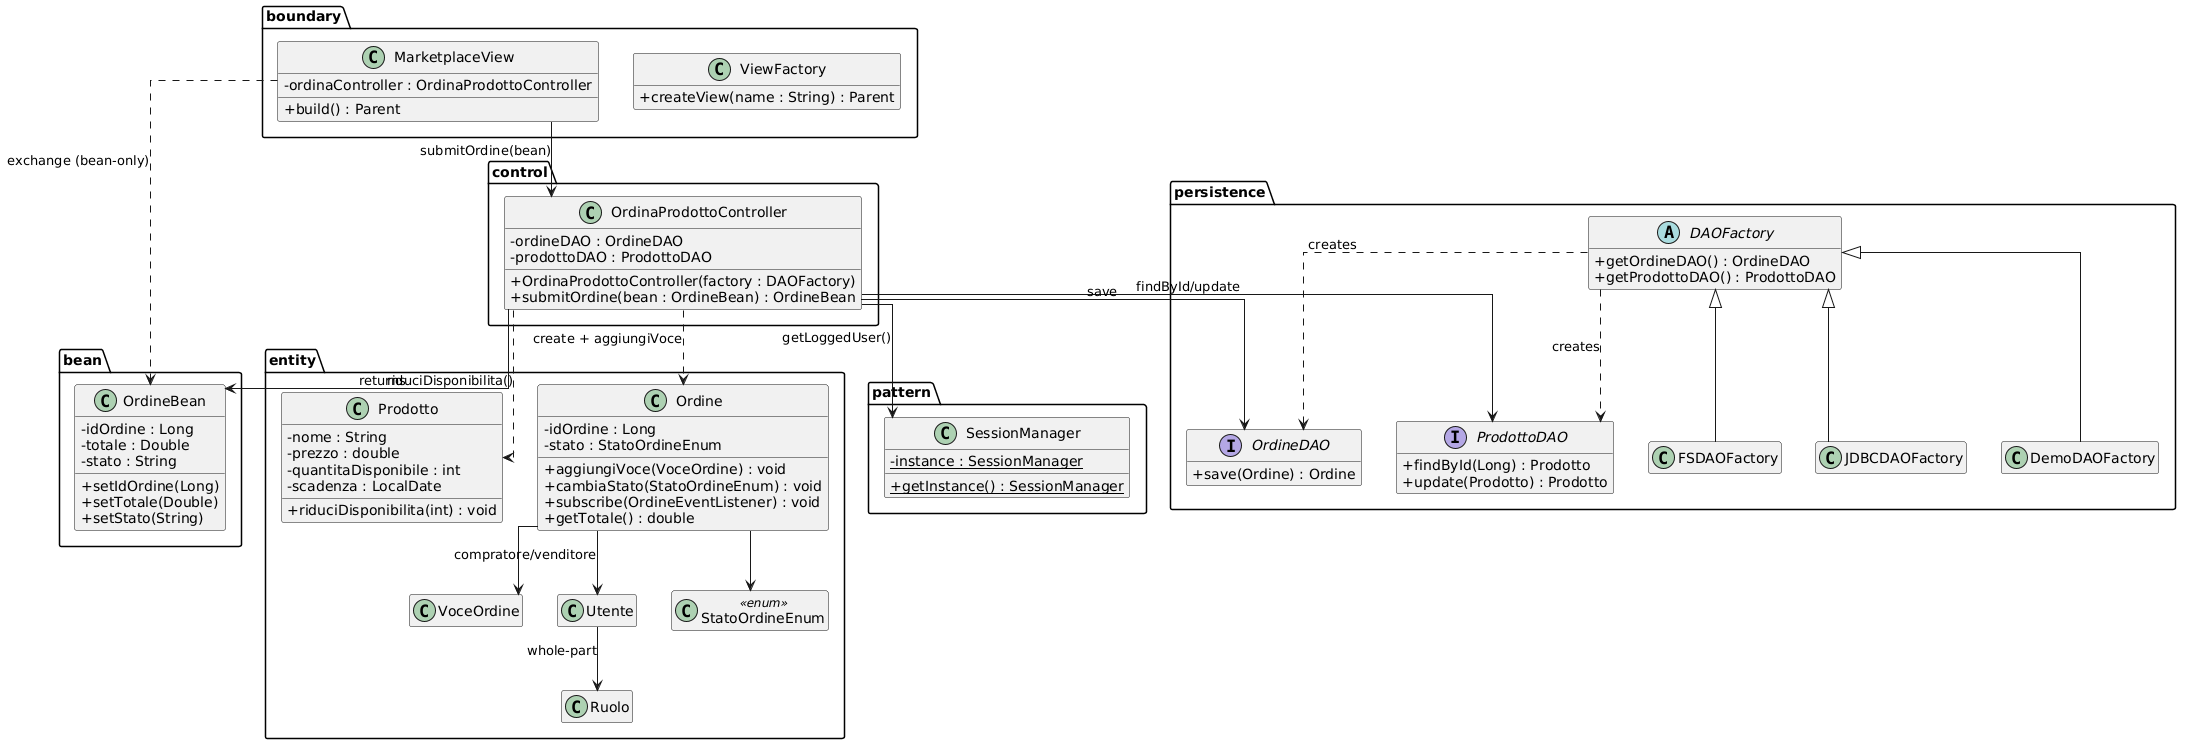
\includegraphics[width=0.98\textwidth]{figures/class-diagram-core.png}
\caption{Design-level class diagram: UC-04 core (boundary/bean/control/entity)
and persistence layer (DAOFactory with Demo/FS/JDBC concrete factories).}
\label{fig:classdiagram}
\end{figure}

\section{GoF Patterns}

\begin{itemize}
    \item \textbf{Singleton} -- \texttt{SessionManager},
    \texttt{ApplicationModeManager}: single session and application mode;
    \item \textbf{Abstract Factory} -- \texttt{DAOFactory} with
    \texttt{DemoDAOFactory}, \texttt{FSDAOFactory}, \texttt{JDBCDAOFactory}:
    coherent family of DAOs switchable at startup (NFR-01);
    \item \textbf{Strategy} -- \texttt{StrictMatchingStrategy},
    \texttt{SubstitutionMatchingStrategy}: interchangeable matching algorithms;
    \item \textbf{Facade} -- \texttt{RicettaMatchingFacade}: single entry
    point to the recipe engine;
    \item \textbf{Observer} -- \texttt{OrdineSubject},
    \texttt{UtenteNotifier}, \texttt{VenditoreNotifier}: order-state
    notifications;
    \item \textbf{Adapter} -- \texttt{OpenFoodFactsAdapter},
    \texttt{JakartaMailAdapter}: isolates external systems;
    \item \textbf{Whole-Part} -- \texttt{Utente} aggregates \texttt{Ruolo}
    (dynamic role metamorfosi, D-02).
\end{itemize}

\section{Activity Diagram (UC-04)}

\begin{figure}[H]
\centering
\begin{tikzpicture}[node distance=1.2cm]
\tikzstyle{act}=[rectangle,draw,minimum width=2.2cm,minimum height=0.7cm]
\node[act] (s1) {Select product};
\node[act,right of=s1,xshift=2.6cm] (s2) {Verify availability};
\node[diamond,draw,right of=s2,xshift=2.4cm,aspect=2] (d1) {quantity available?};
\node[act,below of=d1] (s3) {Show insufficient quantity error};
\node[act,below of=s2,yshift=-2.4cm] (s4) {Show order summary};
\node[act,right of=d1,xshift=2.2cm] (s5) {Confirm order};
\node[diamond,draw,right of=s5,xshift=2.2cm,aspect=2] (d2) {confirmed?};
\node[act,below of=d2] (s6) {Abort};
\node[act,right of=d2,xshift=2.4cm] (s7) {Record order (CREATED)};
\node[act,right of=s7,xshift=2.2cm] (s8) {Notify vendor (async)};
\node[act,below of=s8] (s9) {End};
\draw[->] (s1)--(s2); \draw[->] (s2)--(d1);
\draw[->] (d1)--node[left]{no}(s3); \draw[->] (s3)--(s1);
\draw[->] (d1)--node[above]{yes}(s4); \draw[->] (s4)--(s5);
\draw[->] (s5)--(d2); \draw[->] (d2)--node[left]{no}(s6);
\draw[->] (d2)--node[above]{yes}(s7); \draw[->] (s7)--(s8); \draw[->] (s8)--(s9);
\end{tikzpicture}
\caption{Activity diagram of UC-04 (simplified).}
\label{fig:activity}
\end{figure}

\section{Sequence Diagram (UC-04)}

\begin{figure}[H]
\centering
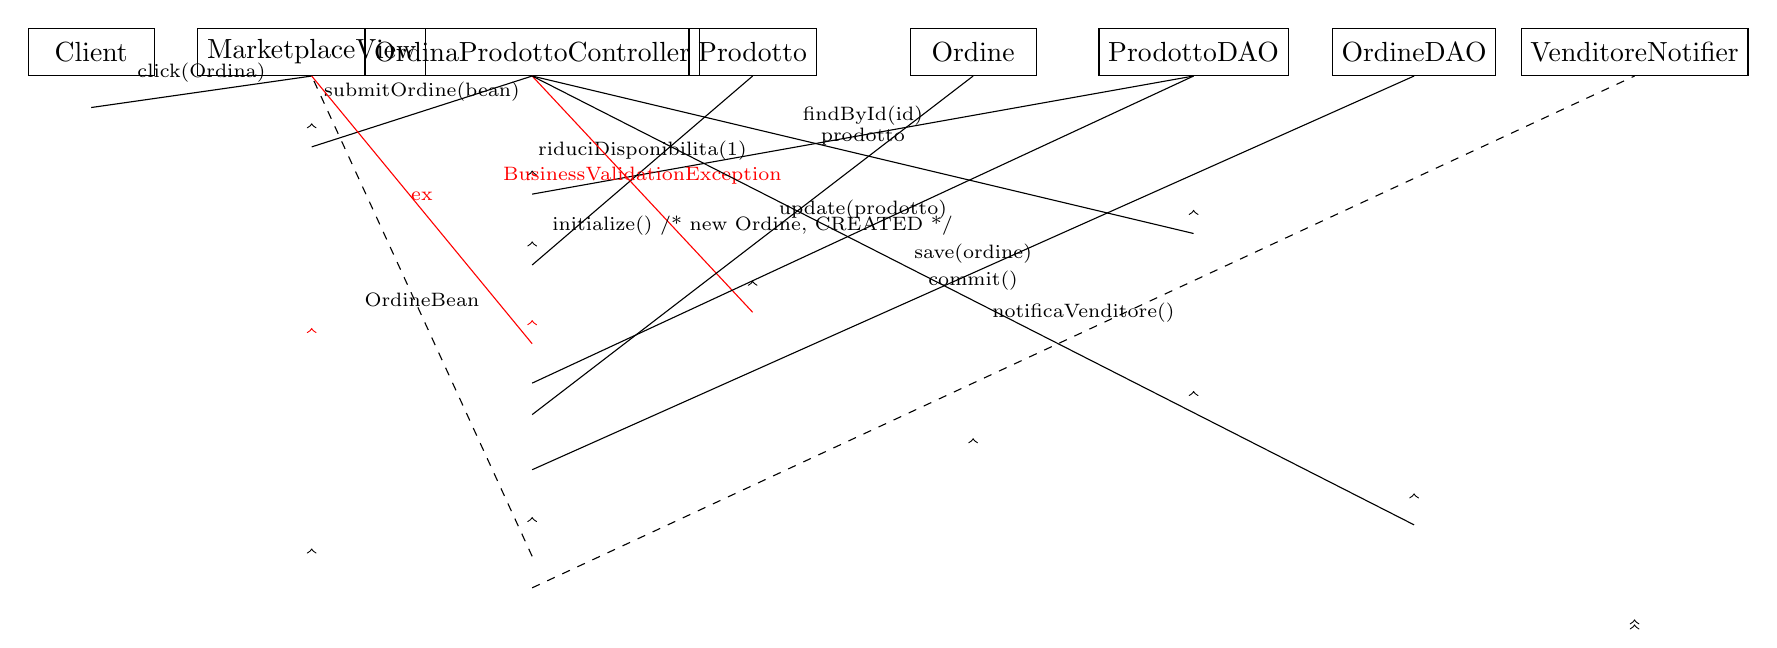
\begin{tikzpicture}
\tikzstyle{inst}=[rectangle,draw,minimum width=1.6cm,minimum height=0.6cm]
\node[inst] (c) {Client};
\node[inst,right of=c,xshift=1.8cm] (b) {MarketplaceView};
\node[inst,right of=b,xshift=1.8cm] (ctl) {OrdinaProdottoController};
\node[inst,right of=ctl,xshift=1.8cm] (pr) {Prodotto};
\node[inst,right of=pr,xshift=1.8cm] (e) {Ordine};
\node[inst,right of=e,xshift=1.8cm] (pdao) {ProdottoDAO};
\node[inst,right of=pdao,xshift=1.8cm] (odao) {OrdineDAO};
\node[inst,right of=odao,xshift=1.8cm] (not) {VenditoreNotifier};
\draw[dashed] (c)--(c.south)+(0,-4.2); \draw[dashed] (b)--(b.south)+(0,-4.2);
\draw[dashed] (ctl)--(ctl.south)+(0,-4.2); \draw[dashed] (pr)--(pr.south)+(0,-4.2);
\draw[dashed] (e)--(e.south)+(0,-4.2); \draw[dashed] (pdao)--(pdao.south)+(0,-4.2);
\draw[dashed] (odao)--(odao.south)+(0,-4.2); \draw[dashed] (not)--(not.south)+(0,-4.2);
% sync messages (full arrows)
\draw[->] (c.south)+(0,-0.4) -- (b.south)+(0,-0.6) node[midway,above]{\scriptsize click(Ordina)};
\draw[->] (b.south)+(0,-0.9) -- (ctl.south)+(0,-1.2) node[midway,above]{\scriptsize submitOrdine(bean)};
\draw[->] (ctl.south)+(0,-1.5) -- (pdao.south)+(0,-1.7) node[midway,above]{\scriptsize findById(id)};
\draw[->] (pdao.south)+(0,-2.0) -- (ctl.south)+(0,-2.1) node[midway,above]{\scriptsize prodotto};
\draw[->] (ctl.south)+(0,-2.4) -- (pr.south)+(0,-2.6) node[midway,above]{\scriptsize riduciDisponibilita(1)};
% exception: BusinessValidationException risale alla boundary
\draw[->,red] (pr.south)+(0,-3.0) -- (ctl.south)+(0,-3.1) node[midway,above]{\scriptsize \textcolor{red}{BusinessValidationException}};
\draw[->,red] (ctl.south)+(0,-3.4) -- (b.south)+(0,-3.2) node[midway,above]{\scriptsize \textcolor{red}{ex}};
% transaction: update + save
\draw[->] (ctl.south)+(0,-3.9) -- (pdao.south)+(0,-4.0) node[midway,above]{\scriptsize update(prodotto)};
\draw[->] (ctl.south)+(0,-4.3) -- (e.south)+(0,-4.6) node[midway,above]{\scriptsize initialize() /* new Ordine, CREATED */};
\draw[->] (ctl.south)+(0,-5.0) -- (odao.south)+(0,-5.3) node[midway,above]{\scriptsize save(ordine)};
\draw[->] (odao.south)+(0,-5.7) -- (ctl.south)+(0,-5.6) node[midway,above]{\scriptsize commit()};
% return bean (dashed)
\draw[->,dashed] (ctl.south)+(0,-6.1) -- (b.south)+(0,-6.0) node[midway,above]{\scriptsize OrdineBean};
% async notification (open arrow)
\draw[->>,dashed] (ctl.south)+(0,-6.5) -- (not.south)+(0,-6.9) node[midway,above]{\scriptsize notificaVenditore()};
\end{tikzpicture}
\caption{Sequence diagram of UC-04: synchronous calls (full arrows), return
bean (dashed), exception propagation (red), async Observer notification
(open arrow).}
\label{fig:sequence}
\end{figure}

\section{State Diagram (Ordine, BR-04)}

\begin{figure}[H]
\centering
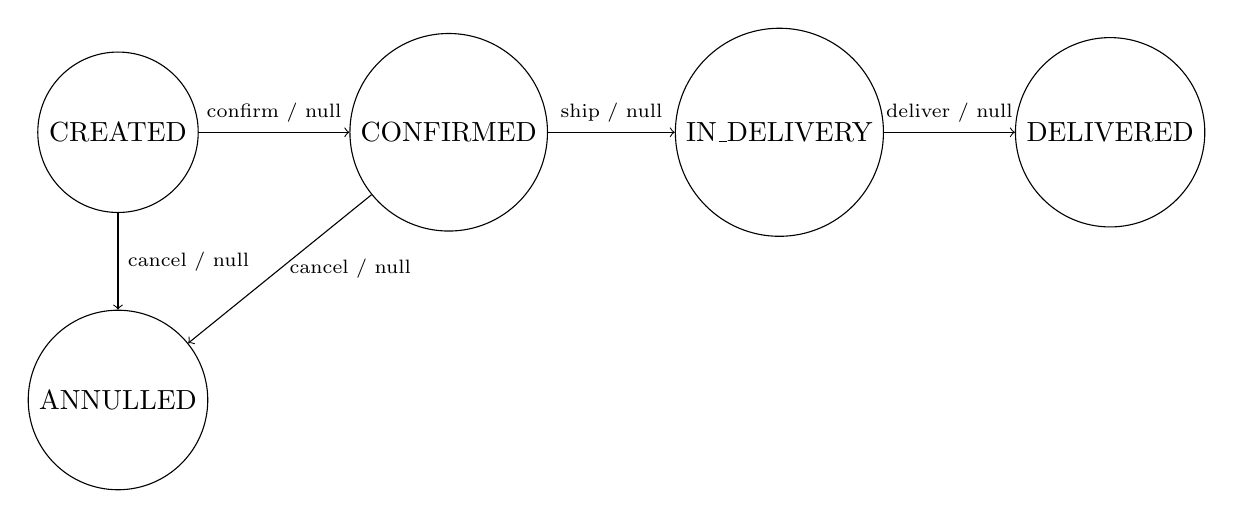
\begin{tikzpicture}[node distance=2cm]
\tikzstyle{st}=[circle,draw,minimum size=1.1cm]
\node[st] (c) {CREATED};
\node[st,right of=c,xshift=2.2cm] (cf) {CONFIRMED};
\node[st,right of=cf,xshift=2.2cm] (in) {IN\_DELIVERY};
\node[st,right of=in,xshift=2.2cm] (del) {DELIVERED};
\node[st,below of=c,yshift=-1.4cm] (an) {ANNULLED};
\draw[->] (c)--(cf) node[midway,above]{\scriptsize confirm / null};
\draw[->] (c)--(an) node[midway,right]{\scriptsize cancel / null};
\draw[->] (cf)--(in) node[midway,above]{\scriptsize ship / null};
\draw[->] (cf)--(an) node[midway,right]{\scriptsize cancel / null};
\draw[->] (in)--(del) node[midway,above]{\scriptsize deliver / null};
\end{tikzpicture}
\caption{State diagram of Ordine (trigger / behaviour, guards mutually
exclusive per BR-04).}
\label{fig:state}
\end{figure}
